\documentclass[12pt, letterpaper]{report} % Usa la clase report para documentos divididos en capítulos

%Paquete que da el formato al documento
\usepackage{pucv_inf_2024}

% Archivo de Referencias
\addbibresource{referencias.bib}

% Glosario
\loadglsentries{glosario}
\makeglossaries

\begin{document}

%% TEX CON PORTADA DEL INFORME
% Portada para informes en asignaturas
\title{Informe\\[0.2cm] Ingeniería de Software}
\author{
	Lucas Contreras - 21.819.471-0\\[0.05cm]
	Eduardo Cordero - 21.595.598-2\\[0.05cm] 
	Daniel Cornejo - 21.628.427-5\\[0.05cm]
	David Henriquez - 21.723.262-7\\[0.05cm]
	Andrés Perez - 21.648.279-4\\[0.05cm]
	Benjamin Sepúlveda - 21.788.222-2\\[0.05cm]
	Constanza Suárez - 21.660..976-k \\[0.05cm]
	}
\date{Junio 2026}

\begin{titlepage}
	\addtocounter{page}{-1} 
	\makeatletter
	\thispagestyle{plain}
	
	\begin{picture}(0,0)
		\put(-102,-80){
\includegraphics[width=21.8cm]{Portadas/imagenes/encabezado}}
	\end{picture}
	
	\begin{flushright} 
		\vspace*{\fill} 
		
		\vspace*{2cm}
		{\textcolor{titlecolor}{\LARGE\bfseries\MakeUppercase{\@title}}}
		
		\vspace*{\fill}
		
		{\textcolor{titlecolor}{\large\bfseries\textsc{
					\@author
		}}} 
	
		\vspace*{0.8cm}
		
		{\textcolor{titlecolor}{\bfseries\textsc{
					Ingeniería de Software\\[0.2cm] 
					\@date
		}}}
		
	\end{flushright}
\end{titlepage}

%% DEDICATORIA (incluir solo en TFT y TFG, sino comentar)
% \include{Dedicatoria/dedicatoria.tex}

%% RESUMEN/ABSTRACT DEL INFORME
% \include{Resumen/resumen.tex}

%% INDICE, LISTAS de FIGURAS/TABLAS/ALGORITMOS, GLOSARIO, ETC.
%% COMENTAR EN CASO DE NO QUERER INCLUIR ALGUNA DE ESTAS LISTAS/INDICES
\newpage\addcontentsline{toc}{chapter}{Índice General}
\tableofcontents % Este comando genera el índice

\newpage\addcontentsline{toc}{chapter}{Lista de Figuras}
\listoffigures % Índice de figuras

\newpage\addcontentsline{toc}{chapter}{Lista de Tablas}
\listoftables  % Índice de tablas

% \newpage\addcontentsline{toc}{chapter}{Lista de Algoritmos\vspace{-0.5cm}}
% \listofalgorithms 

% Lista de Símbolos
% \include{simbolos.tex}
% \newpage\addcontentsline{toc}{chapter}{Lista de Símbolos\vspace{-0.5cm}}
% \printnomenclature

% Imprimir Glosario
% \newpage\addcontentsline{toc}{chapter}{Glosario}
% \printglossary[type=\acronymtype]

\newpage
\pagenumbering{arabic} % Cambia a numeración arábiga para el resto del documento

% CONTENIDO PRINCIPAL DEL DOCUMENTO
\chapter{Introducción}

En la actualidad, la contratación de servicios de flete para el traslado de cargas menores, muebles u objetos personales suele realizarse de manera informal, a través de recomendaciones, contactos directos o publicaciones en redes sociales. Esta situación genera diversas problemáticas para los usuarios, tales como la falta de transparencia en los precios, la dificultad para comparar alternativas, la desconfianza respecto al estado de la carga transportada y la ausencia de mecanismos formales para realizar reclamos o verificar la responsabilidad del transportista.

Frente a esta problemática, el presente proyecto propone el diseño de una plataforma tecnológica orientada a conectar clientes que necesitan realizar traslados con transportistas que ofrecen servicios de flete. El sistema busca facilitar la cotización, contratación, seguimiento y evaluación del servicio, incorporando herramientas que permitan mejorar la seguridad, trazabilidad y confianza entre las partes involucradas. Además, se considera un modelo de negocio basado en una comisión porcentual aplicada a cada viaje completado mediante la plataforma.

Los usuarios principales del sistema son tres: el Cliente, el Transportista y el Administrador. El Cliente podrá solicitar servicios de traslado, comparar transportistas disponibles, revisar precios, realizar pagos, seguir el viaje en tiempo real y calificar el servicio recibido. El Transportista podrá registrarse en la plataforma, configurar sus tarifas, recibir solicitudes cercanas, subir evidencia fotográfica del estado de la carga y gestionar sus servicios realizados. Por su parte, el Administrador tendrá la responsabilidad de validar documentación, gestionar usuarios, revisar reportes y supervisar el funcionamiento general de la plataforma.

La naturaleza del software propuesto corresponde a una aplicación móvil para clientes y transportistas, complementada con un panel web administrativo. Esta combinación permite responder a las necesidades operativas de los usuarios que participan directamente en los traslados, mientras se mantiene una gestión centralizada del sistema por parte de la administración. El software se inspira en plataformas colaborativas de intermediación de servicios, adaptadas específicamente al rubro de los fletes y traslados de carga menor.
En este informe se desarrollan los principales aspectos asociados al proyecto de software, comenzando por el análisis de requerimientos del sistema, donde se identifican las necesidades de los usuarios, los requerimientos funcionales y los requerimientos no funcionales. Posteriormente, se presenta el modelado del sistema mediante diagramas BPMN y casos de uso, junto con la justificación del modelo de desarrollo seleccionado. Además, se describen las herramientas CASE utilizadas, las estrategias de soporte, los aspectos de seguridad y calidad del software, y el diseño de mockups que representan la interfaz propuesta para la plataforma.

Finalmente, este proyecto permite aplicar conceptos fundamentales de la Ingeniería de Software, tales como el levantamiento de requerimientos, el modelado de procesos, la planificación del desarrollo, la documentación técnica y el diseño de soluciones centradas en el usuario. De esta manera, la propuesta busca entregar una solución tecnológica viable, organizada y alineada con las necesidades reales de los usuarios involucrados en la contratación y prestación de servicios de flete.


\chapter{Análisis de requerimientos}
\label{Análisis}

 \section{Descripción del caso de estudio}
 
 El caso de estudio consiste en el diseño y desarrollo de una plataforma tecnológica que conecta de manera eficiente a clientes que necesiten realizar traslados de cargas menores, objetos o muebles, con transportistas que ofrecen sus servicios de flete. La propuesta se inspira en un modelo colaborativo, buscando resolver la falta de transparencia, precios claros y confianza en el rubro.
 
 Para garantizar la seguridad, el sistema cuenta con un mecanismo de verificación visual que obliga al registro fotográfico del estado de la carga al inicio y al final del trayecto, minimizando disputas por daño. El modelo de negocio se sustenta en una comisión porcentual que la plataforma retiene por cada viaje completado.
 
 \section{Requerimientos de usuario}
 
 Los requerimientos de usuario describen lo que los diferentes actores esperan lograr al interactuar con el sistema.
 
 \noindent \textbf{Cliente}
 
 \begin{itemize}
 	\item Necesita cotizar y contratar fletes de forma rápida, conociendo los precios de antemano.
 	\item Requiere visibilidad sobre la calificación del conductor y las características de su vehículo.
 	\item Desea saber en tiempo real dónde se encuentra su carga durante el viaje.
 \end{itemize}
 
 \noindent \textbf{Transportista/Flete}
 
 \begin{itemize}
 	\item Necesita una herramienta o aplicación que le permita recibir solicitudes de trabajo cercanas.
 	\item Requiere definir sus propias tarifas según la distancia y el esfuerzo requerido.
 	\item Necesita un respaldo digital que demuestre que entregó la carga en el mismo estado en que la recibió.
 \end{itemize}
 
 \noindent \textbf{Administrador}
 
 \begin{itemize}
 	\item Necesita herramientas eficaces para validar documentación legal de conductores y vehículos antes de habilitarlos.
 	\item Requiere un panel para resolver dudas, gestionar reportes de usuario y visualizar las métricas financieras del negocio.
 \end{itemize}
 
 \section{Requerimientos funcionales}
 
 \begin{enumerate}
 	\item \textbf{Registro y perfiles}: El sistema debe permitir el registro de tres tipos de usuarios: Cliente, Transportista y Administrador, cada uno con campos de información específicos.
 	\item \textbf{Verificación de documentación}: El sistema debe permitir a los transportistas subir documentos para posteriormente validarlos y recibir la aprobación por parte del Administrador.
 	\item \textbf{Creación de solicitud de traslado}: El sistema debe permitir al Cliente ingresar el origen, destino, tipo de carga, dimensiones, peso aproximado, fecha y hora del servicio.
 	\item \textbf{Motor de búsqueda y comparación}: El sistema debe mostrar al Cliente una lista de transportistas disponibles cercanos, calificación, tipo de vehículo y tiempo de llegada estimado.
 	\item \textbf{Tarifa flexible}: El sistema debe permitir al Transportista configurar y calcular sus tarifas en base a la distancia y las características del traslado.
 	\item \textbf{Registro fotográfico de origen}: El sistema debe obligar al Transportista a tomar y subir fotografías de la carga a la aplicación antes de iniciar el viaje.
 	\item \textbf{Registro fotográfico de destino}: El sistema debe obligar al Transportista a tomar y subir fotografías de la carga al momento de la entrega en el destino.
 	\item \textbf{Almacenamiento de evidencia}: El sistema debe asociar las fotografías tomadas en el origen y destino al historial del servicio correspondiente como respaldo ante posibles reclamos.
 	\item \textbf{Seguimiento en tiempo real mediante GPS}: El sistema debe rastrear la ubicación del Transportista mediante el GPS del dispositivo móvil y mostrarla en un mapa al Cliente durante el servicio.
 	\item \textbf{Chat interno}: El sistema debe proveer un canal de mensajería interno entre el Cliente y el Transportista asignado mientras el servicio esté activo.
 	\item \textbf{Notificaciones SMS}: El sistema debe enviar alertas automáticas en tiempo real al Cliente sobre cambios de estado del viaje.
 	\item \textbf{Gestión de pagos}: El sistema debe procesar pagos integrados y permitir la opción de pago en efectivo.
 	\item \textbf{Gestión de comisiones}: El sistema debe descontar de forma automática la comisión porcentual preestablecida de la plataforma por cada viaje pagado.
 	\item \textbf{Calificaciones y reseñas}: El sistema debe permitir al Cliente calificar y dejar comentarios sobre el desempeño del Transportista una vez finalizado el traslado.
 	\item \textbf{Panel de control administrativo}: El sistema debe proveer al Administrador una interfaz web para bloquear o desbloquear usuarios, gestionar reportes y ver métricas.
 	\item \textbf{Historial de servicios}: El sistema debe mantener un registro accesible para clientes y transportistas con el detalle de todos sus viajes, recibos y estados.
 \end{enumerate}
 
 \section{Requerimientos no funcionales}
 
 Los requerimientos no funcionales definen las restricciones de calidad, rendimiento y propiedades del entorno del software.
 
 \begin{enumerate}
 	\item \textbf{Seguridad de la información}: Todas las comunicaciones y datos sensibles deben estar encriptados.
 	\item \textbf{Disponibilidad}: El sistema y la base de datos deben garantizar una disponibilidad 24/7, minimizando las caídas imprevistas de la aplicación móvil.
 	\item \textbf{Rendimiento y tiempo de respuesta}: Las consultas a los GPS de transportistas cercanos y la actualización del mapa en tiempo real no deben demorar más de 2,67 segundos en refrescarse.
 	\item \textbf{Usabilidad UX/UI}: Las interfaces móviles deben ser intuitivas y responsivas, diseñadas para que un usuario común pueda solicitar un flete en pocos pasos.
 	\item \textbf{Escalabilidad}: El programa debe ser capaz de soportar un incremento concurrente de usuarios sin degradar la plataforma.
 	\item \textbf{Compatibilidad móvil}: La aplicación móvil para clientes y transportistas debe ser compatible con Android e iOS.
 \end{enumerate}
\chapter{Modelado de diagramas de casos de uso}
\label{Modelado de diagramas de casos de uso}

A continuación se mostrarán los diagramas de casos de uso. Para ser concretos, se van a mostrar: Diagrama BPMN que detalla el proceso general de uso de los actores del sistema, y el sistema, Diagrama de Caso de Uso Principal que es una representación gráfica de los actores y casos de uso identificados, y por último la Descripción de Casos de Uso, que es una explicación detallada de cada caso de uso, incluyendo nombre, actores involucrados, flujo principal de eventos, precondiciones y postcondiciones.

\section{Diagrama BPMN}

\begin{figure}[H]
	\centering
	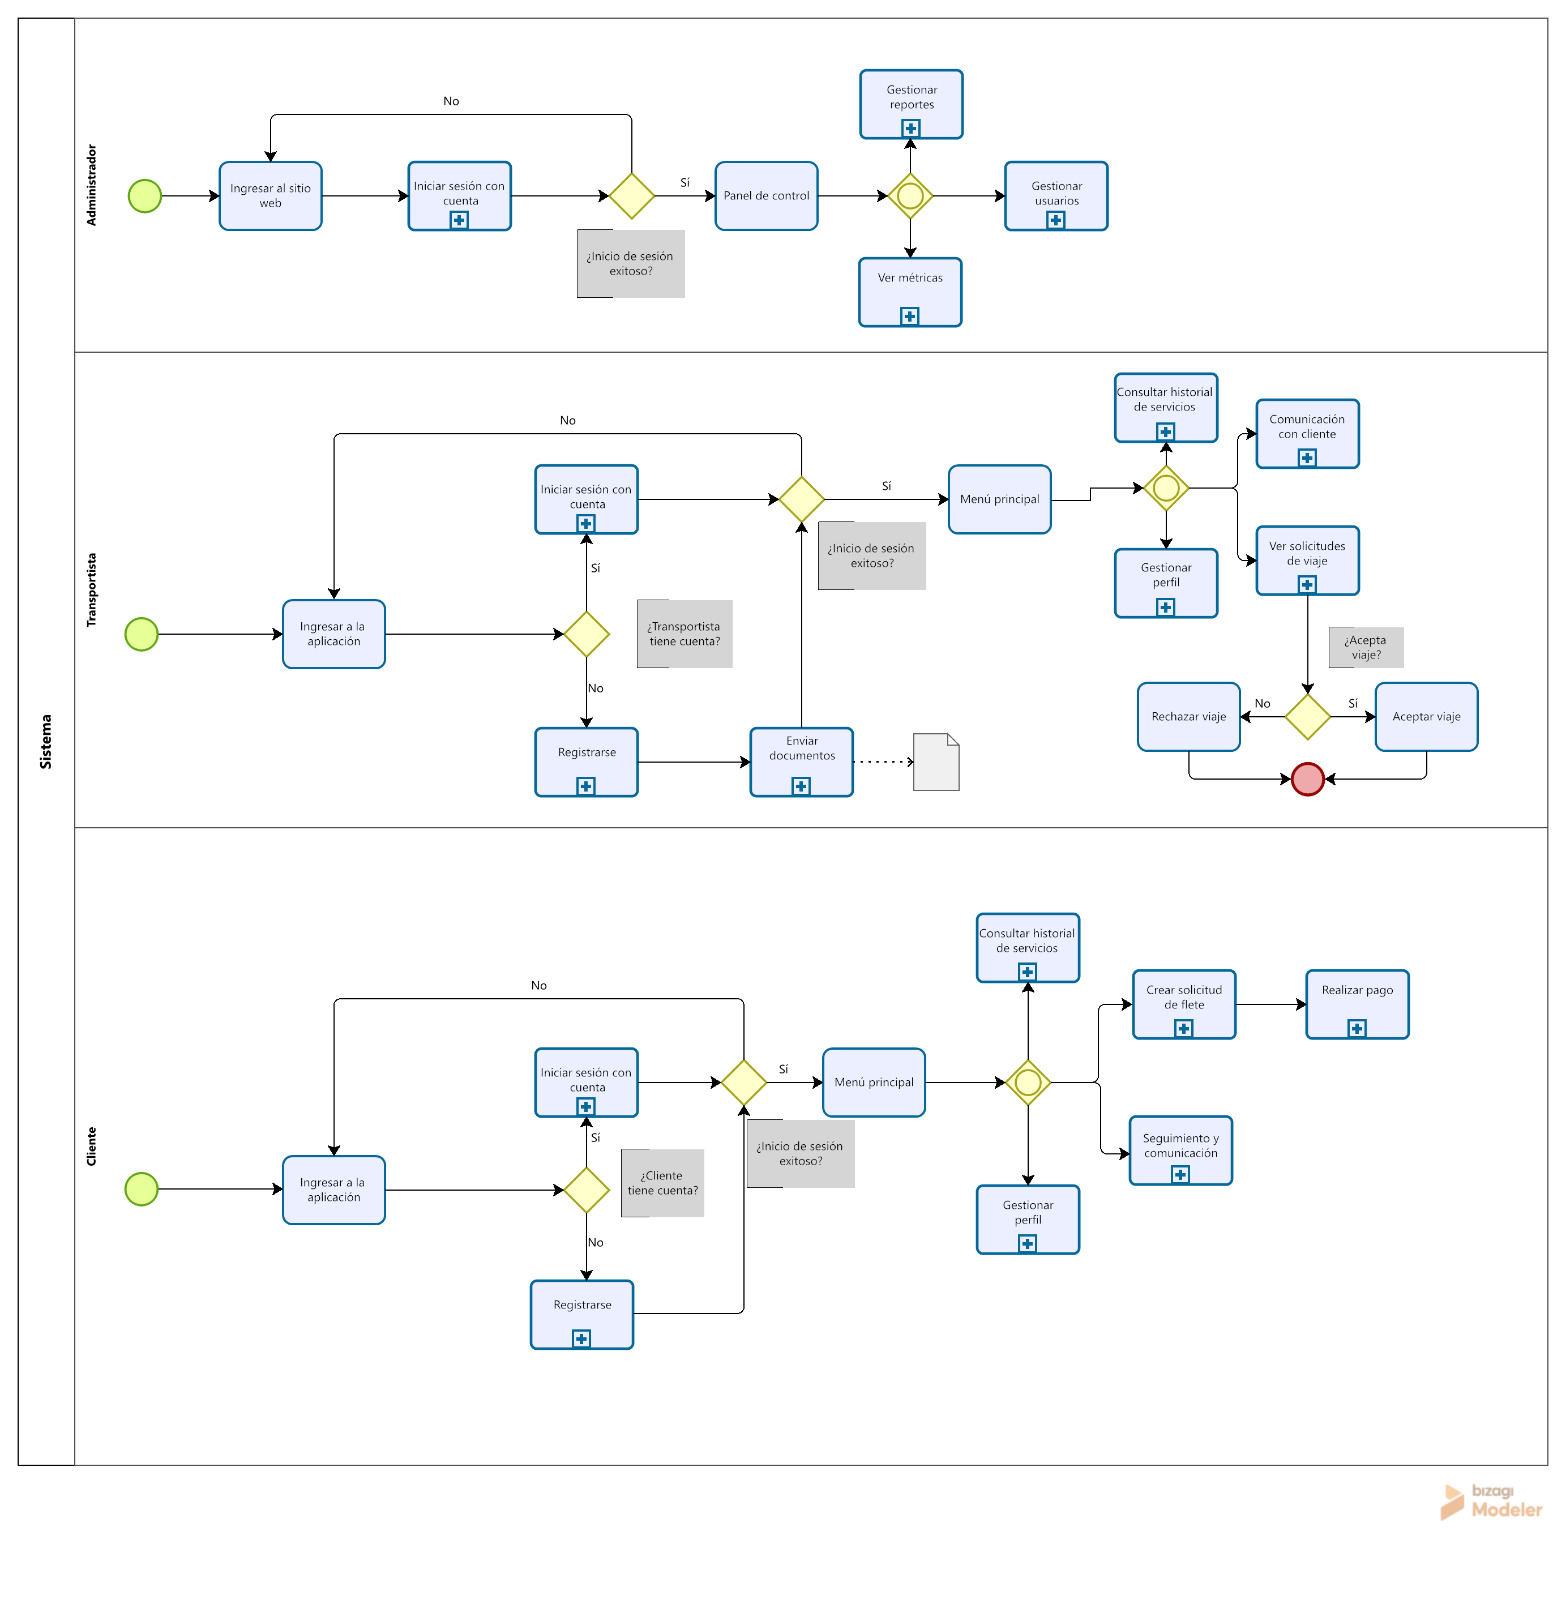
\includegraphics[width=1\linewidth]{Figuras/BPMN.jpeg}
	\caption{Diagrama BPMN del sistema}
	\label{fig:Diagrama BPMN sistema}
\end{figure}

\noindent \textbf{Descripción de cada subproceso}

\noindent \textbf{Administrador:}

\begin{itemize}
	\item Iniciar sesión con cuenta: Subproceso donde el administrador valida sus credenciales (usuario y contraseña). Se revisa en la base de datos que esto sea correcto y se da o no el acceso al panel de control.
	\item Gestionar reportes: Subproceso enfocado en la lectura, seguimiento y resolución de incidencias, dudas o reclamos generados por los clientes o transportistas.
	\item Gestionar usuarios: Subproceso que permite visualizar la lista entera de usuarios registrados, aplicar bloqueos/desbloqueos de cuentas y evaluar los documentos legales de los transportistas que están pendientes de validación para aceptarlos o rechazarlos.
	\item Ver métricas: Subproceso donde el sistema recopila y renderiza estadísticas sobre el uso de la aplicación, estado de los viajes y gráficos financieros con las comisiones retenidas
\end{itemize}

\noindent \textbf{Transportista:}

\begin{itemize}
	\item Registrarse: Subproceso donde el conductor ingresa su información personal y detalla las características de su vehículo.
	\item Enviar documentos: Subproceso obligatorio durante el registro del transportista, en el cual adjunta fotos o escaneos de su documentación para que el administrador pueda revisarlo.
	\item Iniciar sesión con cuenta: Subproceso que valida el estado de la cuenta del transportista (aprobado o bloqueado) y le da acceso al menú principal.
	\item Consultar historial de servicios: Subproceso en el que se consulta a la base de datos todos los fletes realizados, mostrando sus detalles, estados y comprobantes de pago para mostrarlos en pantalla.
	\item Gestionar perfil: Subproceso donde el conductor puede actualizar sus datos de contacto, contraseña y características editables de su perfil público.
	\item Ver solicitudes de viaje: Subproceso donde el transportista recibe alertas de fletes cercanos requeridos y decide aceptar o rechazar la oferta de viaje.
	\item Comunicación con cliente: Subproceso habilitado solo durante un viaje en curso, que provee un chat interno para coordinar los detalles logísticos con el cliente.
	
\end{itemize}

\noindent \textbf{Cliente:}

\begin{itemize}
	\item Registrarse: Subproceso donde el cliente crea su perfil ingresando sus datos básicos de contacto
	\item Iniciar sesión con cuenta: Subproceso que valida las credenciales del cliente y le da acceso al menú principal.
	\item Gestionar perfil: Subproceso donde el usuario puede modificar sus datos de contacto o actualizar su información de acceso.
	\item Consultar historial de servicios: Subproceso que permite revisar el registro de sus fletes solicitados, incluyendo acceso a recibos, detalles del transportista que hizo el viaje y fotografías de evidencia.
	\item Crear solicitud de flete: Subproceso donde el cliente ingresa los parámetros de su necesidad (origen, destino, dimensiones de la carga, etc.). Luego, el sistema busca conductores cercanos y el cliente selecciona una opción para generar el contrato de viaje.
	\item Seguimiento y comunicación: Subproceso en tiempo real que renderiza la ubicación GPS del vehículo en un mapa, gestiona el envío automático de notificaciones por cambios de estado y habilita el chat con el conductor.
	\item Realizar pago: Subproceso donde el cliente abona el servicio (mediante tarjeta o efectivo). El sistema registra la transacción, descuenta la comisión correspondiente y habilita el formulario para calificar al transportista.
\end{itemize}


\section{Diagrama de caso de uso general}

\begin{figure}[htbp]
	\centering
	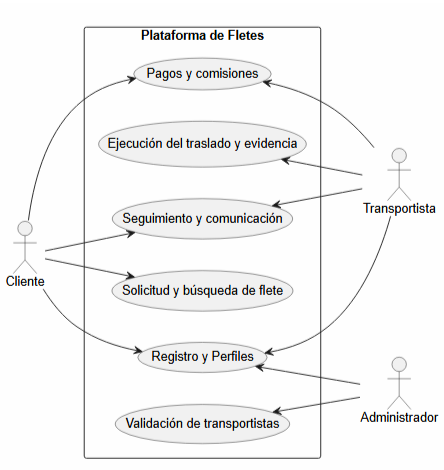
\includegraphics[width=0.5\linewidth]{Figuras/DiagramaDeCasoGeneralizado.png}
	\caption{Diagrama de caso generalizado}
	\label{fig:Diagrama de caso generalizado}
\end{figure}
\newpage

\begin{figure}[H]
	\centering
	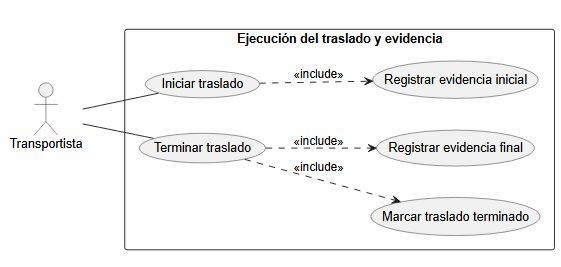
\includegraphics[width=0.7\linewidth]{Figuras/DiagramaTrasladoEvidencia.png}
	\caption{Diagrama de caso de uso: Traslado y evidencia}
	\label{fig:Diagrama traslado y evidencia}
\end{figure}

\begin{table}[H]
	\centering 
	\caption{Tabla explicativa del caso de traslado y evidencia}
	\label{table: Tabla caso traslado y evidencia}
	\renewcommand{\arraystretch}{1.4}
	\begin{tabular}{|p{4cm}|p{11cm}|}
		\hline
		\centering\textbf{Elemento} & \centering\textbf{Descripción}\tabularnewline
		\hline
		\textbf{Nombre} & Ejecución del traslado y evidencia \\
		\hline 
		\textbf{Requerimientos asociados} & RF6, RF7, RF8 \\
		\hline
		\textbf{Actor principal} & Transportista \\
		\hline
		\textbf{Actores secundarios} & Sistema \\
		\hline
		\textbf{Precondiciones} & El servicio debe estar contratado y el transportista debe haber aceptado o tener asignado el traslado. La aplicación debe permitir el uso de cámara o carga de fotografías. \\
		\hline
		\textbf{Flujo principal} & 
		1. El transportista llega al punto de origen. \newline
		2. Antes de iniciar el traslado, el sistema solicita registrar fotografías de la carga. \newline
		3. El transportista toma y sube fotografías del estado inicial de la carga. \newline
		4. El sistema almacena las fotografías y las asocia al servicio correspondiente. \newline
		5. El transportista inicia el traslado. \newline
		6. Al llegar al destino, el sistema solicita un nuevo registro fotográfico. \newline
		7. El transportista toma y sube fotografías del estado final de la carga. \newline
		8. El sistema guarda la evidencia final en el historial del servicio. \newline
		9. El transportista marca la entrega como finalizada. \\
		\hline
		\textbf{Postcondiciones} & 
		- El servicio queda respaldado con evidencia fotográfica de origen y destino. \newline
		- Las fotografías quedan almacenadas en el historial del viaje y pueden 
		ser consultadas ante reclamos, dudas o disputas por daños \\
		\hline
	\end{tabular} 
\end{table}

\begin{figure}[H]
	\centering
	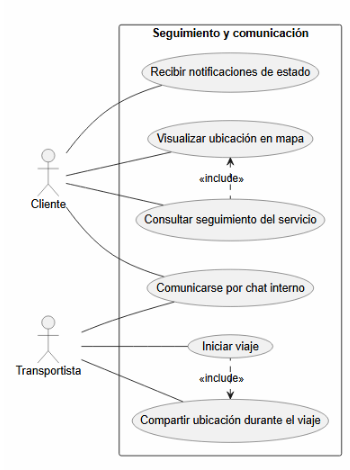
\includegraphics[width=0.4\linewidth]{Figuras/DiagramaSeguimientoComunicacion.png}
	\caption{Diagrama de caso de uso: Seguimiento y comunicación}
	\label{fig:Diagrama seguimiento y comunicación}
\end{figure}

\begin{table}
	\centering 
	\caption{Tabla explicativa del caso de seguimiento y comunicación}
	\label{table: Tabla caso seguimiento y comunicación}
	\renewcommand{\arraystretch}{1.4}
	\begin{tabular}{|p{4cm}|p{11cm}|}
		\hline
		\centering\textbf{Elemento} & \centering\textbf{Descripción}\tabularnewline
		\hline
		\textbf{Nombre} & Seguimiento y comunicación \\
		\hline 
		\textbf{Requerimientos asociados} & RF9, RF10, RF11 \\
		\hline
		\textbf{Actor principal} & Cliente \\
		\hline
		\textbf{Actores secundarios} & Transportista, Sistema \\
		\hline
		\textbf{Precondiciones} & El servicio debe estar contratado y activo. El transportista debe permitir el uso de ubicación GPS en su dispositivo móvil. El cliente debe tener acceso al detalle del viaje y un número telefónico registrado para recibir notificaciones SMS. \\
		\hline
		\textbf{Flujo principal} & 
		1. El transportista inicia el viaje desde la aplicación. 
		2. El sistema obtiene periódicamente la ubicación GPS del transportista. 
		3. El cliente ingresa al seguimiento del servicio y visualiza la ubicación en un mapa. 
		4. Durante el servicio, cliente y transportista pueden comunicarse mediante el chat interno. 
		5. Cuando ocurre un cambio relevante de estado, como inicio del viaje, llegada al destino o finalización, el sistema genera una notificación automática. 
		6. El sistema envía la alerta al cliente mediante SMS. \\
		\hline
		\textbf{Postcondiciones} & 
		- El cliente puede conocer la ubicación aproximada de su carga durante el traslado. \newline
		- La comunicación entre cliente y transportista queda centralizada en la plataforma. \newline
		- El cliente recibe avisos relevantes sobre el avance del servicio. \\
		\hline
	\end{tabular} 
\end{table}

\newpage

\begin{figure}[H]
	\centering
	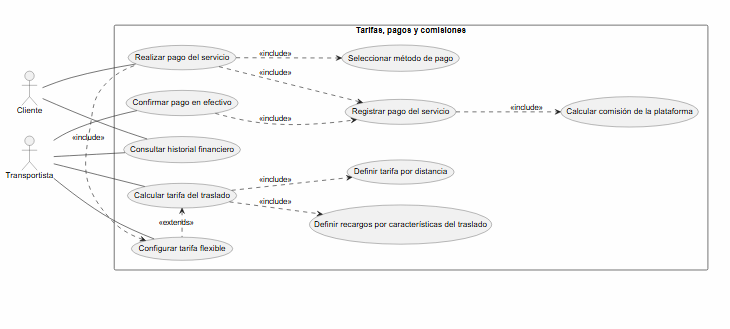
\includegraphics[width=1\linewidth]{Figuras/DiagramaTarifaPagoComisiones.png}
	\caption{Diagrama de tarifa y pago de comisiones}
	\label{fig: Diagrama tarifa}
\end{figure}



\begin{table}
	\centering 
	\caption{Tabla explicativa del caso de pagos y comisiones}
	\label{table: Tabla caso pagos y comisiones}
	\renewcommand{\arraystretch}{1.4}
	\begin{tabular}{|p{4cm}|p{11cm}|}
		\hline
		\centering\textbf{Elemento} & \centering\textbf{Descripción}\tabularnewline
		\hline
		\textbf{Nombre} & Pagos y comisiones \\
		\hline 
		\textbf{Requerimientos asociados} & RF5, RF12, RF13 \\
		\hline
		\textbf{Actor principal} & Transportista, Sistema \\
		\hline
		\textbf{Actores secundarios} & Transportista, Sistema \\
		\hline
		\textbf{Precondiciones} & El transportista debe tener una cuenta activa y estar habilitado para ofrecer servicios. El servicio debe estar contratado o finalizado, según la regla de pago definida por la plataforma. La tarifa del traslado debe poder calcularse a partir de la distancia y las características del servicio. La plataforma debe tener definida una comisión porcentual. \\
		\hline
		\textbf{Flujo principal} & 
		1. El transportista configura su tarifa flexible según distancia y características del traslado. \newline
		2. El sistema registra la configuración tarifaria del transportista. \newline
		3. El cliente accede al pago del servicio.\newline
		4. El sistema calcula el monto del traslado usando la tarifa configurada por el transportista.\newline
		5. El sistema muestra el monto total a pagar al cliente.\newline
		6. El cliente selecciona el método de pago disponible: tarjeta o efectivo.\newline
		7. El cliente realiza el pago.\newline
		8. El sistema registra el pago asociado al servicio.\newline
		9. El sistema calcula la comisión porcentual de la plataforma. \newline
		10. El sistema descuenta o registra la comisión según el método de pago utilizado. \newline
		11. El sistema actualiza el estado financiero del viaje. \\
		\hline
		\textbf{Postcondiciones} & 
		La tarifa del traslado queda calculada según la configuración del transportista. El pago queda registrado en el sistema. La comisión de la plataforma queda calculada y asociada al servicio. El viaje queda disponible para historial, recibos y métricas financieras administrativas \\
		\hline
	\end{tabular} 
\end{table} 

\newpage

\begin{figure}[H]
	\centering
	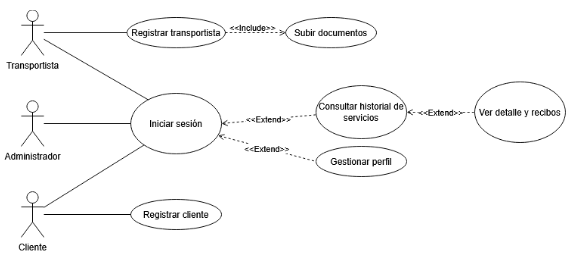
\includegraphics[width=0.7\linewidth]{Figuras/DiagramaRegistroPerfiles.png}
	\caption{Diagrama de caso de uso: Registro y perfiles}
	\label{fig:Diagrama registro y perfiles }
\end{figure}

\begin{table}
	\centering 
	\caption{Tabla explicativa del caso de registro y perfiles}
	\label{table: Tabla caso registro y perfiles}
	\renewcommand{\arraystretch}{1.4}
	\begin{tabular}{|p{4cm}|p{11cm}|}
		\hline
		\centering\textbf{Elemento} & \centering\textbf{Descripción}\tabularnewline
		\hline
		\textbf{Nombre} & Registro y perfiles \\
		\hline 
		\textbf{Requerimientos asociados} & RF1, RF2 (parcialmente), RF16 \\
		\hline
		\textbf{Actor principal} & Cliente, Transportista, Administrador \\
		\hline
		\textbf{Actores secundarios} & Sistema \\
		\hline
		\textbf{Precondiciones} & El usuario debe tener acceso a la plataforma (aplicación móvil o interfaz web (Administrador)). En el caso de querer consultar el historial y/o editar los datos, el usuario debe haber iniciado sesión en el sistema. \\
		\hline
		\textbf{Flujo principal} & 
		1. El usuario selecciona la opción de registro según el rol que le corresponda (Cliente o Transportista). \newline 
		2. El usuario ingresa los datos específicos que se requieran para su perfil. \newline 
		3. En el caso del Transportista, el sistema lo obliga a adjuntar su documentación legal (licencia, vehículo, etc.) antes de continuar. \newline 
		4. El sistema valida la consistencia de los datos, crea la cuenta y permite al nuevo usuario ingresar a la plataforma. \newline 
		5. El usuario ingresa a la sección de configuración para gestionar o actualizar los datos de su perfil. \newline 
		6. El usuario (Cliente o Transportista) revisa su historial de servicios desde el menú. \newline 
		7. El sistema busca y encuentra el registro de todos los servicios asociados al usuario. \newline 
		8. El sistema muestra en pantalla el listado con el detalle, recibos de pago y los estados históricos de cada servicio. \\
		\hline
		\textbf{Postcondiciones} & 
		- El nuevo usuario queda registrado y clasificado según su rol en la plataforma. \newline 
		- Los documentos del transportista quedan almacenados y disponibles para que el administrador los revise. \newline 
		- Los datos modificados en el perfil se actualizan en la base de datos. \newline 
		- El historial de servicios queda disponible para consultas por parte de los clientes y transportistas. \\
		\hline
	\end{tabular} 
\end{table}

\newpage

\begin{figure}[H]
	\centering
	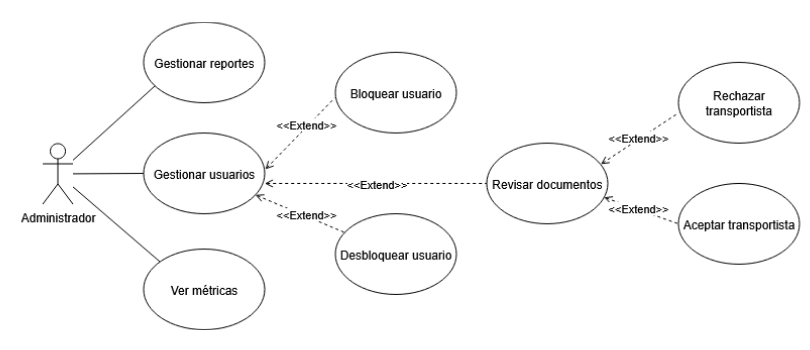
\includegraphics[width=0.8\linewidth]{Figuras/DiagramaTransportistasControl.png}
	\caption{Diagrama de caso de uso: Validación transportistas y control administrativo}
	\label{fig:Diagrama transportistas y control administrativo }
\end{figure}

\begin{table}
	\centering 
	\caption{Tabla explicativa del caso de validación de transportistas y control administrativo}
	\label{table: Tabla caso validación de transportistas y control administrativo}
	\renewcommand{\arraystretch}{1.4}
	\begin{tabular}{|p{4cm}|p{11cm}|}
		\hline
		\centering\textbf{Elemento} & \centering\textbf{Descripción}\tabularnewline
		\hline
		\textbf{Nombre} & Validación de transportistas y control administrativo \\
		\hline 
		\textbf{Requerimientos asociados} & RF2 (parcialmente), RF15 \\
		\hline
		\textbf{Actor principal} & Administrador \\
		\hline
		\textbf{Actores secundarios} & Sistema \\
		\hline
		\textbf{Precondiciones} & El administrador debe estar logueado en la plataforma web. Para la revisión de documentos, deben existir cuentas de transportistas pendientes de aprobación. \\
		\hline
		\textbf{Flujo principal} & 
		1. El administrador accede al panel de control y selecciona una de las tres áreas de gestión disponibles: Reportes, Usuarios o Métricas. \newline 
		2. Si elige gestionar reportes, el sistema muestra las incidencias o dudas enviadas por los usuarios para resolverlas o gestionarlas. \newline 
		3. Si elige ver métricas, el sistema muestra los gráficos financieros, las comisiones retenidas y las estadísticas de uso del negocio. \newline 
		4. Si elige gestionar usuarios, el sistema muestra una lista con todos los clientes y transportistas. \newline 
		5. Desde la gestión de usuarios, el administrador puede seleccionar un perfil para bloquear o desbloquear un usuario de la plataforma según corresponda. \newline 
		6. Desde la misma lista, el administrador puede seleccionar un transportista que se encuentre pendiente para la revisión de documentos. \newline 
		7. El sistema despliega los archivos adjuntos por el transportista para su validación. \newline 
		8. El administrador evalúa la documentación y decide si acepta o no al transportista. \\
		\hline
		\textbf{Postcondiciones} & 
		- Las cuentas de los transportistas cambian su estado (aprobado, rechazado o bloqueado). \newline 
		- Los usuarios bloqueados pierden el acceso a la aplicación de forma inmediata. \newline 	
		- Los reportes gestionados actualizan su estado de resolución y las métricas se mantienen al día. \\
		\hline
	\end{tabular} 
\end{table}

\newpage

\begin{figure}[H]
	\centering
	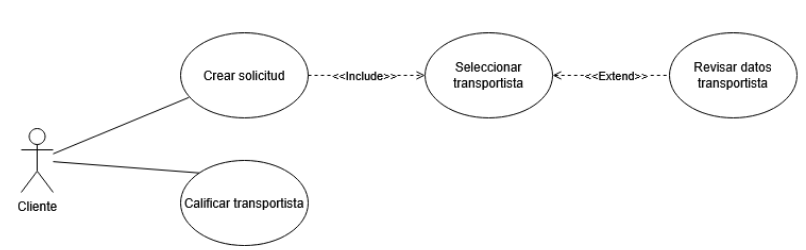
\includegraphics[width=0.8\linewidth]{Figuras/DiagramaSolicitudBusquedaFlete.png}
	\caption{Diagrama de caso de uso: Solicitud y búsqueda de flete}
	\label{fig:Diagrama solicitud y búsqueda de flete }
\end{figure}

\begin{table}
	\centering 
	\caption{Tabla explicativa del caso de solicitud y búsqueda de flete}
	\label{table: Tabla caso solicitud y búsqueda de flete}
	\renewcommand{\arraystretch}{1.4}
	\begin{tabular}{|p{4cm}|p{11cm}|}
		\hline
		\centering\textbf{Elemento} & \centering\textbf{Descripción}\tabularnewline
		\hline
		\textbf{Nombre} & Solicitud y búsqueda de flete \\
		\hline 
		\textbf{Requerimientos asociados} & RF3, RF4, RF14 \\
		\hline
		\textbf{Actor principal} & Cliente \\
		\hline
		\textbf{Actores secundarios} & Sistema \\
		\hline
		\textbf{Precondiciones} & El cliente debe estar autenticado en la aplicación móvil. Para calificar al transportista, el servicio de traslado debe estar finalizado. \\
		\hline
		\textbf{Flujo principal} & 
		1. El cliente inicia el proceso seleccionando la opción para crear una nueva solicitud de traslado. \newline 
		2. El cliente ingresa el origen, destino, tipo de carga, dimensiones, peso aproximado, fecha y hora de servicio. \newline 
		3. El sistema procesa los datos y activa el motor de búsqueda para localizar transportistas disponibles y cercanos. \newline 
		4. El sistema muestra al cliente un listado de los transportistas sugeridos, detallando su calificación y tipo de vehículo. \newline 
		5. El cliente puede seleccionar opcionalmente un transportista de la lista para revisar su perfil completo y comentarios de otros clientes. \newline 
		6. El cliente selecciona al transportista que prefiere y confirma el envío de la solicitud de flete. \newline 
		7. Tras haberse completado el traslado, el sistema habilita la opción de evaluación para el cliente. \newline 
		8. El cliente clasifica el desempeño del transportista mediante un sistema de estrellas y puede redactar una reseña escrita en caso de así desearlo. \\
		\hline
		\textbf{Postcondiciones} & 
		- La solicitud de traslado queda registrada en el sistema y asociada al transportista seleccionado para que éste pueda iniciar el viaje. \newline
		- Se guardan las calificaciones y comentarios del cliente, actualizando la evaluación general del transportista en la plataforma. \\
		\hline
	\end{tabular} 
\end{table}






\printbibliography[title={Referencias}]

\end{document}
